\begin{figure}[tb]
  \centering
  \begin{subfigure}{0.19\linewidth}
  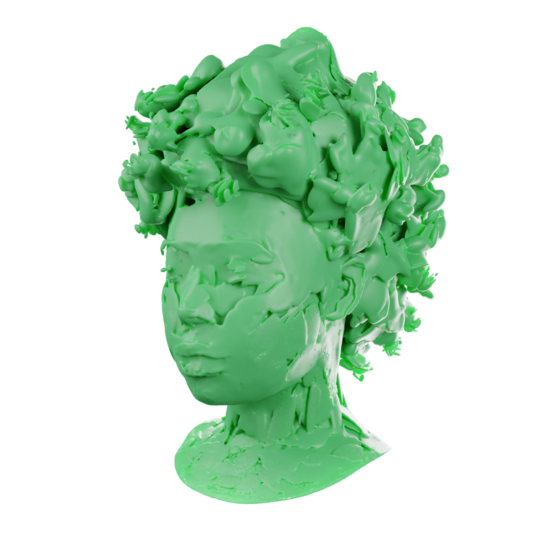
\includegraphics[width=\linewidth]{images/meshes/khady_sugar.png}
  \end{subfigure}
  %
  \hfill
  %
  \begin{subfigure}{0.19\linewidth}
  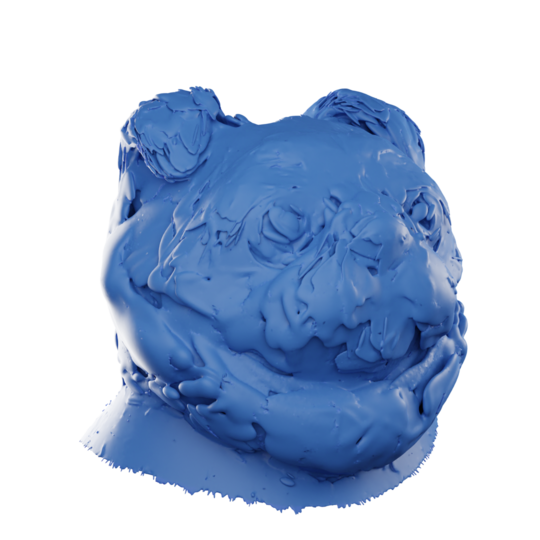
\includegraphics[width=\linewidth]{images/meshes/pug_sugar.png}
  \end{subfigure}
  %
  \hfill
  %
  \begin{subfigure}{0.19\linewidth}
  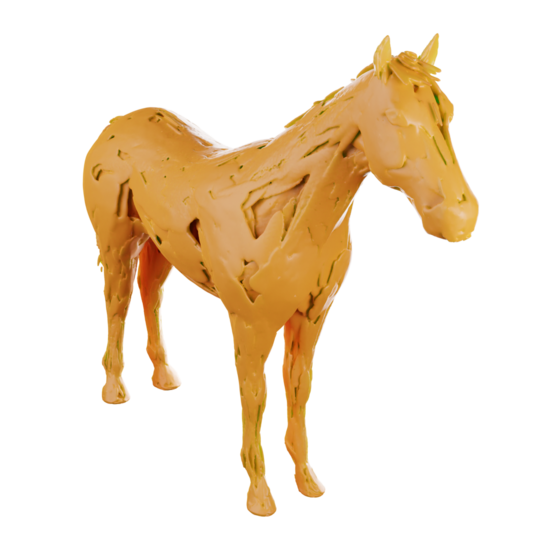
\includegraphics[width=\linewidth]{images/meshes/horse_y_sugar.png}
  \end{subfigure}
  %
  \hfill
  %
  \begin{subfigure}{0.19\linewidth}
  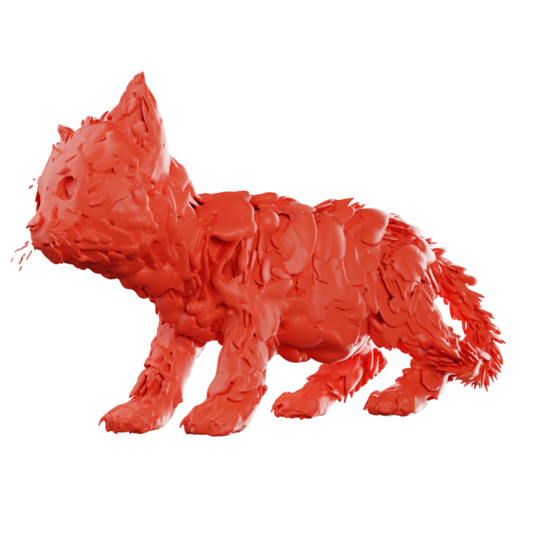
\includegraphics[width=\linewidth]{images/meshes/kitten_sugar.png}
  \end{subfigure}
  %\hfill
  %
  % \begin{subfigure}{0.19\linewidth}
  % \includegraphics[width=\linewidth]{images/meshes/woolly_sugar.png}
  % \end{subfigure}
  %
  %
  \vspace{0.005\linewidth}\\
  {\small (a) Using the predefined, large parameter $D$ as in SuGaR~\cite{guedon2023sugar}} 
  % \vspace{0.01\linewidth}
  \\
  %
  \begin{subfigure}{0.19\linewidth}
  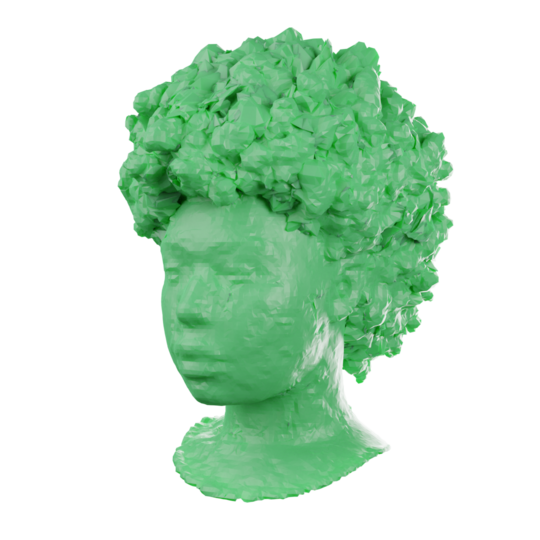
\includegraphics[width=\linewidth]{images/meshes/khady_frosting.png}
  \end{subfigure}
  %
  \hfill
  %
  \begin{subfigure}{0.19\linewidth}
  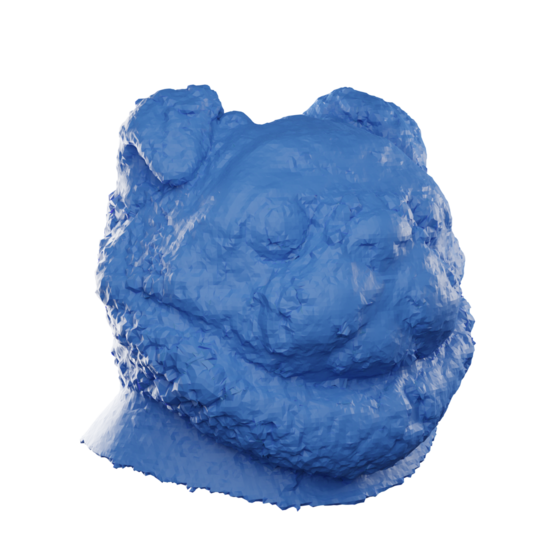
\includegraphics[width=\linewidth]{images/meshes/pug_frosting.png}
  \end{subfigure}
  %
  \hfill
  %
  \begin{subfigure}{0.19\linewidth}
  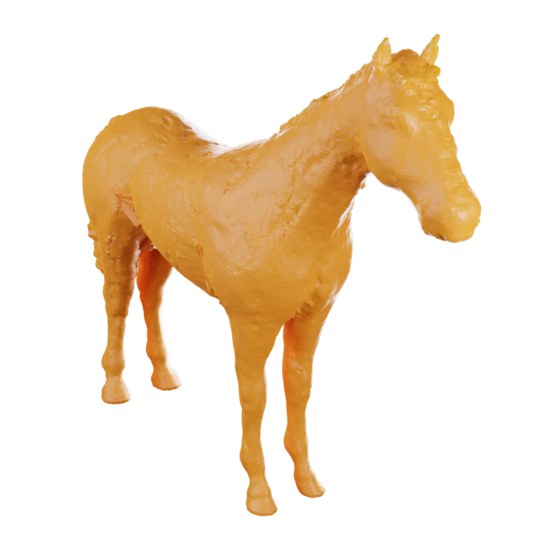
\includegraphics[width=\linewidth]{images/meshes/horse_y_frosting.png}
  \end{subfigure}
  %
  \hfill
  %
  \begin{subfigure}{0.19\linewidth}
  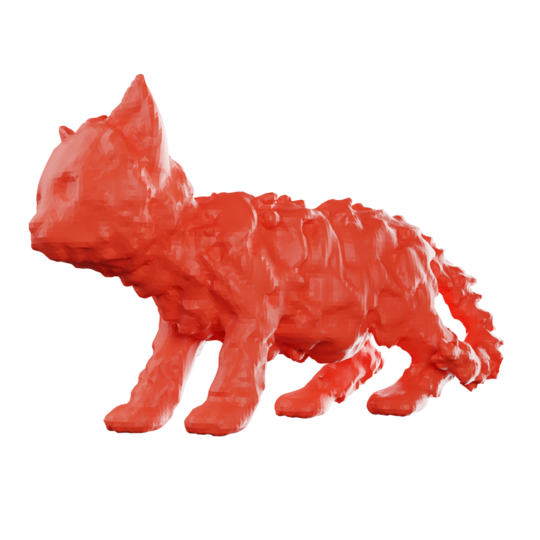
\includegraphics[width=\linewidth]{images/meshes/kitten_frosting.png}
  \end{subfigure}
  %
  % \hfill
  % %
  % \begin{subfigure}{0.19\linewidth}
  % \includegraphics[width=\linewidth]{images/meshes/woolly_frosting.png}
  % \end{subfigure}
  %
  % \vspace{0.005\linewidth}
  \\
  {\small (b) Using our automatically computed $D$ that adapts to the complexity of the 3DGS}
  %
  \caption{
  \textbf{Comparison of meshes extracted by SuGaR from the Shelly dataset without and with our improvement that automatically tunes the octree depth $D$ in Poisson reconstruction depending on the complexity of the scene.}
  Our technique~(bottom) drastically reduces surface artifacts for many scenes, such as the holes and the ellipsoidal bumps on the surface when using the default values from~\cite{guedon2023sugar}~(top).
}
  % \vincentrmk{I would remove the purple thing on the right, the 2 meshes are not very different}
%  \vincentrmk{I removed the wooly thing}
  % Moreover, the outer bound of the frosting layer~(bottom), which is computed using the unconstrained, non-aligned Gaussians, generally provides a refined mesh with better quality than the mesh directly obtained from the isosurface of the aligned Gaussians.
  
  
    % \textbf{Comparison of meshes reconstructed from Gaussian Splatting representations using SuGaR~\cite{guedon2023sugar} and our approach.}
  % Our method to compute automatically optimal hyperparameters for Poisson recontruction~(center) drastically reduces surface artifacts for a lot of scenes, such as the ellipsoidal bumps on the surface when using the default values from~\cite{guedon2023sugar}~(left). Moreover, the outer bound of the frosting layer~(right), which is computed using the unconstrained, non-aligned Gaussians, generally provides a refined mesh with better quality than the mesh directly obtained from the isosurface of the aligned Gaussians.}}
  \label{fig:mesh-comparison}
\end{figure}
% \todo{We also follow SuGaR~\cite{guedon2023sugar} for extracting a base mesh, but we can actually give more details as shown above. Indeed, SuGaR is very elusive on this part; I think it's interesting to understand what Poisson reconstruction provides, that the density functions lacks. Moreover, this part may be important to explain the improvement that I a added, which is a way to automatically compute the optimal octree depth hyperparameter for Poisson reconstruction depending on the configuration of the Gaussians in the scene. This greatly helps to remove "blobs" in the scene without having to tweak the octree depth parameter by hand, so it could be a contribution. Having a well-balanced mesh is important to get a nice frosting.}